\documentclass[a4paper]{article}

%------------------------------------------------------------
\usepackage[a4paper, total={6in, 9in}]{geometry}
\usepackage{amsmath, amssymb}
\usepackage{booktabs}
\usepackage{caption}
\usepackage{enumitem}
\usepackage{graphicx}
\usepackage{float}
\usepackage{inconsolata}
\usepackage{listings}
\usepackage{mathtools}
\usepackage{pstricks-add}
\usepackage{siunitx}
\usepackage[most]{tcolorbox}
\usepackage{tikz, pgfplots}
\usepackage{epstopdf} %converting to PDF
\usepackage{hyperref}
\usepackage{xfrac}

\usetikzlibrary{shapes.geometric}
\usetikzlibrary{arrows}
\usetikzlibrary{calc}

%------------------------------------------------------------
\graphicspath{{./fig/}}
\pgfplotsset{compat=1.13}
%------------------------------------------------------------
\setlength{\parindent}{0in}

\lstdefinestyle{C++}{
	language=C++,
	basicstyle=\ttfamily,
	keywordstyle=\color{blue}\ttfamily,
	stringstyle=\color{red}\ttfamily,
	commentstyle=\color{green}\ttfamily,
	morecomment=[l][\color{magenta}]{\#},
	showstringspaces=false
}

%------------------------------------------------------------
\newtcblisting[auto counter]{sexylisting}[2][]{sharp corners, 
    fonttitle=\bfseries, colframe=gray, listing only, 
    listing options={basicstyle=\ttfamily,language=C++}, 
    title=Listing \thetcbcounter: #2, #1}

%------------------------------------------------------------
\lstset{language=C++,
        basicstyle=\ttfamily,
        keywordstyle=\color{blue}\ttfamily,
        stringstyle=\color{red}\ttfamily,
        commentstyle=\color{green}\ttfamily,
        morecomment=[l][\color{magenta}]{\#},
        showstringspaces=false
}
%------------------------------------------------------------
\tikzstyle{block} = [draw, fill=blue!20, rectangle, 
    minimum height=3em, minimum width=3em]
\tikzstyle{sum} = [draw, fill=blue!20, circle, node distance=1cm]
\tikzstyle{input} = [coordinate]
\tikzstyle{output} = [coordinate]
\tikzstyle{pinstyle} = [pin edge={to-,thin,black}]

%------------------------------------------------------------
\newlength{\arrow}
\settowidth{\arrow}{\scriptsize$1000$}

\newcommand*{\myrightarrow}[1]{\xrightarrow{\mathmakebox[\arrow]{#1}}}

\newcommand{\uvec}[1]{\boldsymbol{\hat{\textbf{#1}}}}

%------------------------------------------------------------

\begin{document}
\title{ENG252 Dynamics: Practical 3}
\author{Shane Reynolds}
\maketitle

\section{Introduction}
\subsection{Moment of Inertia}
Consider a body with mass $m$ undergoing rotational motion, with angular acceleration $\alpha$, around a fixed axis $OO'$. Graphically this scenario is depicted in Figure 1. If we want to calculate the Moment of this body around the axis $OO'$, then we need to consider the moments of each and every infinitesimally small mass particle that make up the body. The moment of a single particle mass is given by:
\begin{equation}
M = \boldsymbol{r} \times \boldsymbol{F}
\end{equation}

We note $\boldsymbol{r}$ is the position vector of the particle from point where the moment is to calculated, and $\boldsymbol{F}$ is the force acting on the particle. If our motion is constrained to a 2D plane, equation (1) simplifies to the well known equation:
\begin{equation}
M = F \times d
\end{equation}
The quantity $F$ is the scalar magnitude of the force acting orthogonal to the shortest line connecting the particle mass to the moment point of calculation; and $d$ is the distance between between these two points. Using (2) we can calculate the moment $M_O$ about axis $OO'$ for a small mass element, $dm$, of the body in Figure 1:
\begin{equation}
	M_O = Fr = a_t \ dm \ r 
\end{equation}

\begin{figure}[h]
	\centering
	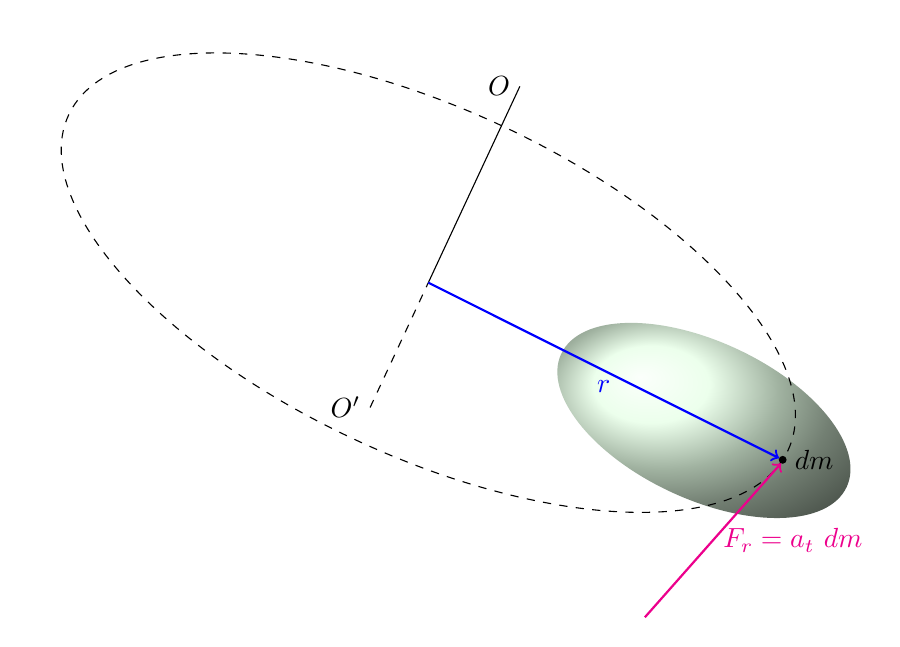
\begin{tikzpicture}
		\shade[ball color=green!10!, rotate=-25] (0,0) coordinate(C) ellipse (2 and 1);
		\fill[color=black] (1,-0.5) circle (0.05); 
		\draw[rotate around={-25:(-3.5,1.75)}] (-3.5,1.75) -- (-3.5,4.5) node[left] (1) {$O$};
		\draw[dashed, rotate around={-25:(-3.5,1.75)}] (-3.5,0) node[left] (2) {$O'$} -- (-3.5,1.75);
		\draw[->, color=blue, thick] (-3.5,1.75) -- (0.9546,-0.4788) node [midway, below] {$r$};
		\draw [dashed, rotate around={-25:(-3.5,1.75)}] (-3.5,1.75) ellipse (5.04 and 2.2);
		\draw [->, color=magenta, thick] (-0.75,-2.5) -- (0.9788,-0.545) node [midway, right] {$F_r = a_t \ dm$};
		\node at (1.4,-0.5) {$dm$};
	\end{tikzpicture}
	\caption{A body of mass $m$ rotating about a fixed axis $OO'$ with some angular acceleration $\alpha$.}
\end{figure}

According to Giancoli \cite{Giancoli:2000} a particle undergoing fixed axis rotation can re-express tangential acceleration $a_t$, as $\alpha r$, where $r$ is the distance from the centre of rotation to the particle. We can now rite (3) as:
\begin{equation}
M_O = \alpha r \ dm \ r
\end{equation}

This is convenient since $\alpha$ remains constant for all infinitesimally small particles in the body meaning that the only variable that needs consideration is $r$. In fact, to calculate the sum of the moments of the body around axis $OO'$ we need to integrate the right hand side of equation (4), which yields:
\begin{equation}
\sum M_O = \alpha \int r^2 dm
\end{equation}

Equation (5) is often thought of as somewhat analogous to $\sum F = ma$, but for rotational motion. In fact since $\alpha$ is the angular acceleration, the integral in equation (5) is often referred to as the resistance of a body to change it's state of rotation. In the literature this quantity is denoted $I$ and referred to as the Moment of Inertia and is defined as:
\begin{equation}
I = \int r^2 dm
\end{equation}

For a body with a uniform mass density $\rho$, we note that $dm = \rho dV$, where $dV$ is an infinitesimally small volume located a distance of $r$ from the centre of rotation. Equation (6) can be written as:
\begin{equation}
I = \rho \int r^2 dV 
\end{equation}

Equation (7) is deceptively simple, however, the evaluation of $I$ can be fiendishly difficult for axes of rotation which do not pass through the body's centre of mass. In practice, (7) is typically only used to determine the moment of inertia through the body's mass centre, $I_G$. To find a moment of inertia around an axis that does not pass through the mass centre, the parallel axis theorem is often applied. The theorem derivation is beyond the scope of this paper, however, the result can be seen in equation (8) \cite{Giancoli:2000}.
\begin{equation}
I_O = I_G + md^2
\end{equation}

Equation (8) tells us if the moment of inertia around an axis passing through the mass centre of a body $I_G$ is known, then the moment of inertia around any parallel axis $I_O$ is calculated with an additive translation of $I_G$ by the body mass $m$ multiplied by the square of orthogonal Euclidean distance between the two axes $d$.

\subsection{Radius of Gyration}
Meriam and Kraige \cite{Meriam:2000} define the radius of gyration $k$ as the radial distance from some axis of rotation such that if the whole mass of the body were concentrated to a point, then the moment of inertia about the given axis would be identical in value to the moment of inertia about the axis using the actual distribution of the body's mass. Mathematically, for some mass $m$, if $I_O$ is the moment of inertia about some axis $O$ then the radius of gyration is defined as:
\begin{equation}
k = \sqrt{\frac{I_O}{m}}
\end{equation}

The radius of gyration has a similar parallel axes theorem as that seen for moments of inertia in equation (8). If we know the radius of gyration for the axis passing through the mass centre, $k_G$, then a parallel axis $O$ at distance $d$ has radius of gyration given by:
\begin{equation}
	k^2_O = k^2_G + d^2
\end{equation}

\subsection{Determining Moments of Inertia with a Trifilar}
A Trifilar is a simple apparatus used to determine an object's Mass Moment of Inertia. The device consists of a circular platform with some mass $m$, which is suspended by three wire filaments of length $L$. Filaments are placed at 120$^o$ separation from each other, at a distance of $r_F$ from the disk centre. An object is placed in the centre of the device to determine it's mass moment of interia. Figure 2 shows an unloaded Trifilar disk in a state of rotation.

\begin{figure}[h]
	\centering
	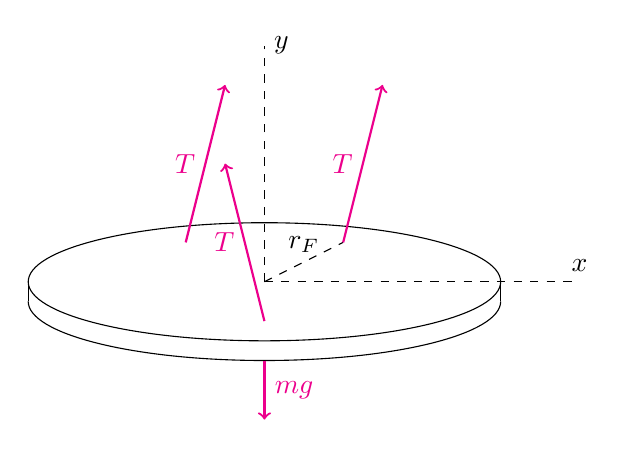
\begin{tikzpicture}
	\draw (0,0) ellipse (3 and 0.75);
	\draw (-3,-0.25) arc (180:360:3 and 0.75);
	\draw (-3,0) -- (-3,-0.25);
	\draw (3,0) -- (3,-0.25);
	\draw [dashed] (0,0) -- (0,3) node [right] {$y$};
	\draw [dashed] (0,0) -- (4,0) node [above] {$x$};
	\draw [dashed] (0,0) -- (1,0.5) node [midway, above] {$r_F$};
	\draw [->, thick, color=magenta] (1,0.5) -- (1.5,2.5) node [midway, left] {$T$};
	\draw [->, thick, color=magenta] (-1,0.5) -- (-0.5,2.5) node [midway, left] {$T$};
	\draw [->, thick, color=magenta] (0,-0.5) -- (-0.5, 1.5) node [midway, left] {$T$};
	\draw [->, thick, color=magenta] (0,-1) -- (0, -1.75) node [midway, right] {$mg$};
	\end{tikzpicture}
	\caption{A Trifilar is a simple apparatus used to determine the moment of inertia for different objects.}
\end{figure}

If the disk is given some initial rotational perturbation, the interaction between the weight of the disk $mg$, and the forces from the filaments $T$ cause a rotational motion. An expression for natural frequency of oscillation $f_n$ of the disk and object can be derived by considering the sum of forces in the vertical direction and the moments about the disk centre. The derivation is beyond the scope of this paper, however, the result can be seen in equation (11) below:
\begin{equation}
f_n = \frac{r_F}{2 \pi k} \sqrt{\frac{g}{L}}
\end{equation}

An object's moment of inertia is found by placing it on the disk, and perturbing the disk such that it only undergoes rotational motion, oscillating about the disk centre. Natural oscillation frequency can be determined by observing period of oscillation $T_n$ for the disk and object and applying equation (12) below:
\begin{equation}
f_n = \frac{1}{T_n}
\end{equation}

Rearranging (11) allows for the radius of gyration to be expressed as a function of $f_n$, $r$, and $L$:
\begin{equation}
k = \frac{r_F}{2 \pi f_n} \sqrt{\frac{g}{L}}
\end{equation}

Equating equations (12) and (13) allows us to solve for the mass moment of inertia about the mass centre:
\begin{equation}
	I = \frac{mg}{L} \bigg( \frac{r_F}{2 \pi f_n} \bigg)^2
\end{equation}

\newpage

\subsection{Scope}
This practical requires the Mass Moment of Inertia to be determined for various objects, using a trifilar. The first object is a wooden disk, which makes up part of the trifilar; and the second object is a small bolt like mass. The trifilar apparatus can be seen in Figure 3; and the bolt like mass is shown in Figure 4. To determine the Mass Moment of Inertia, the trifilar will be rotationally perturbed and natural periods of oscillation will be observed. Captured experimental data will be used to calculate the moment of inertia, which will then be compared to the theoretically derived results.
\begin{figure}[h]
	\centering
	\begin{minipage}{0.45\textwidth}
		\centering
		\frame{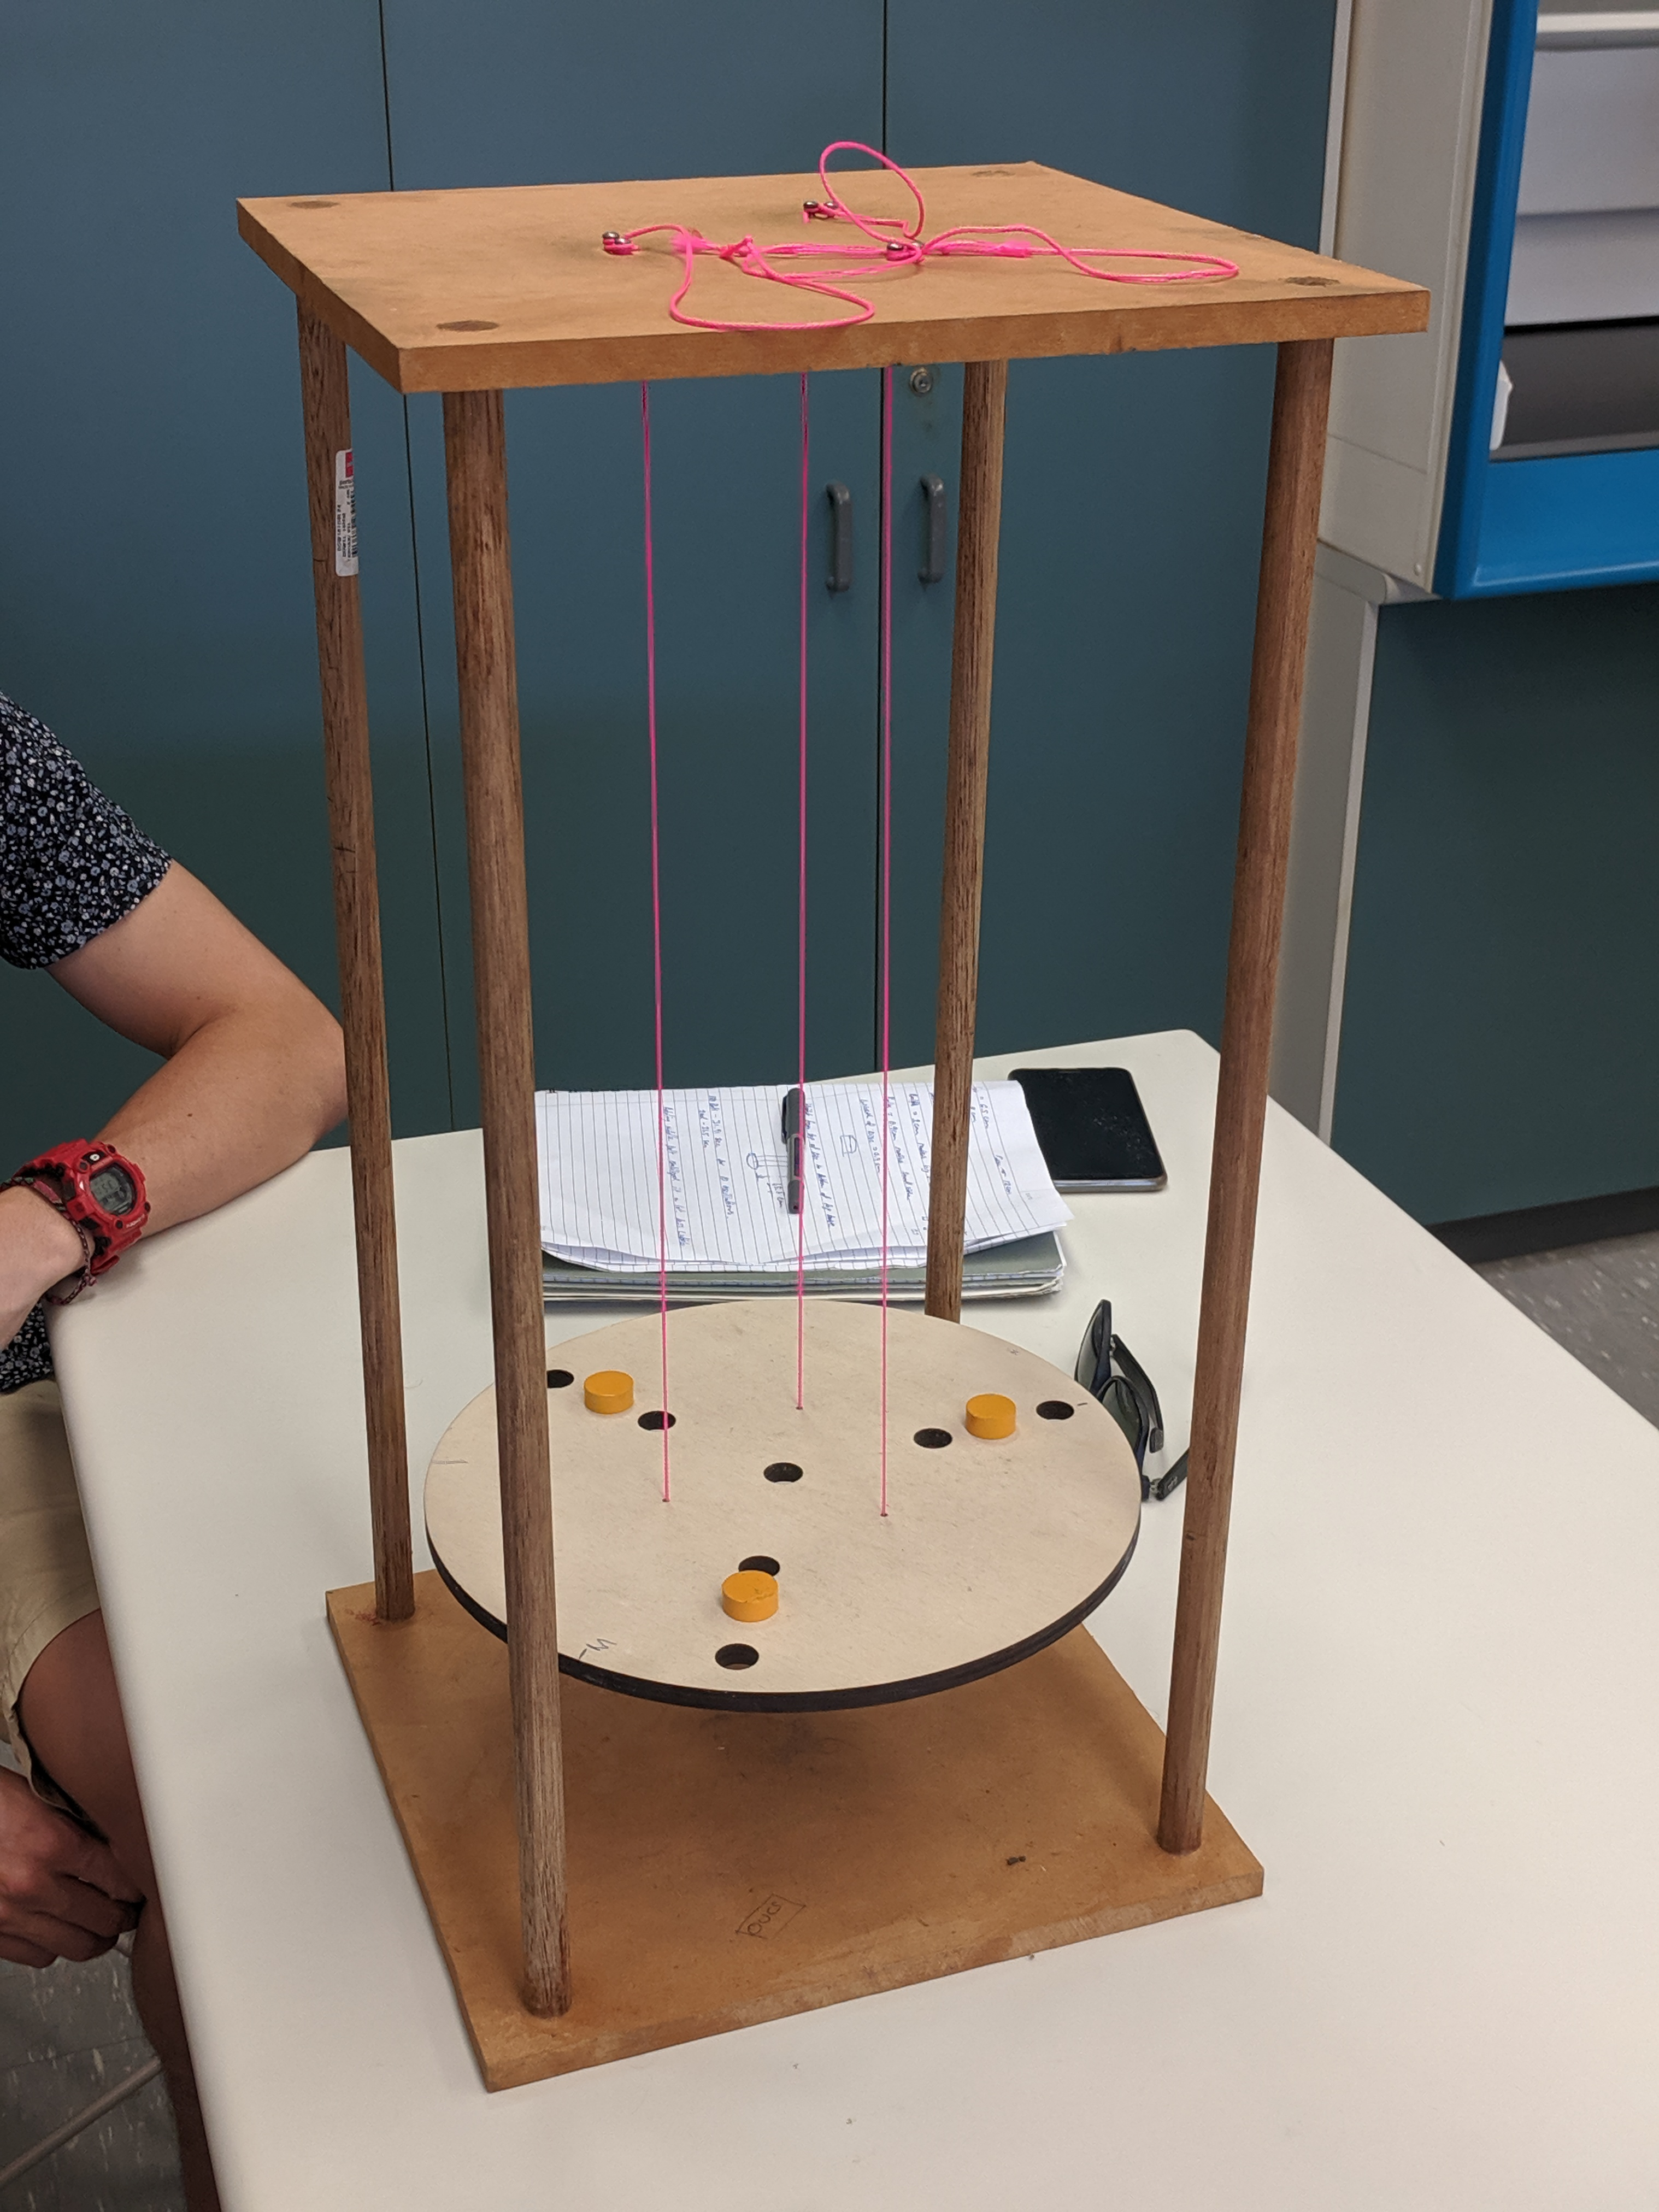
\includegraphics[scale=0.05]{scope_1}}
		\caption{The trifilar rig consists of a wooden disk suspended by three filament wires. Masses can be placed in holes provided that are in the disk.}
	\end{minipage}
	\hspace{1cm}
	\begin{minipage}{0.45\textwidth}
		\centering
		\frame{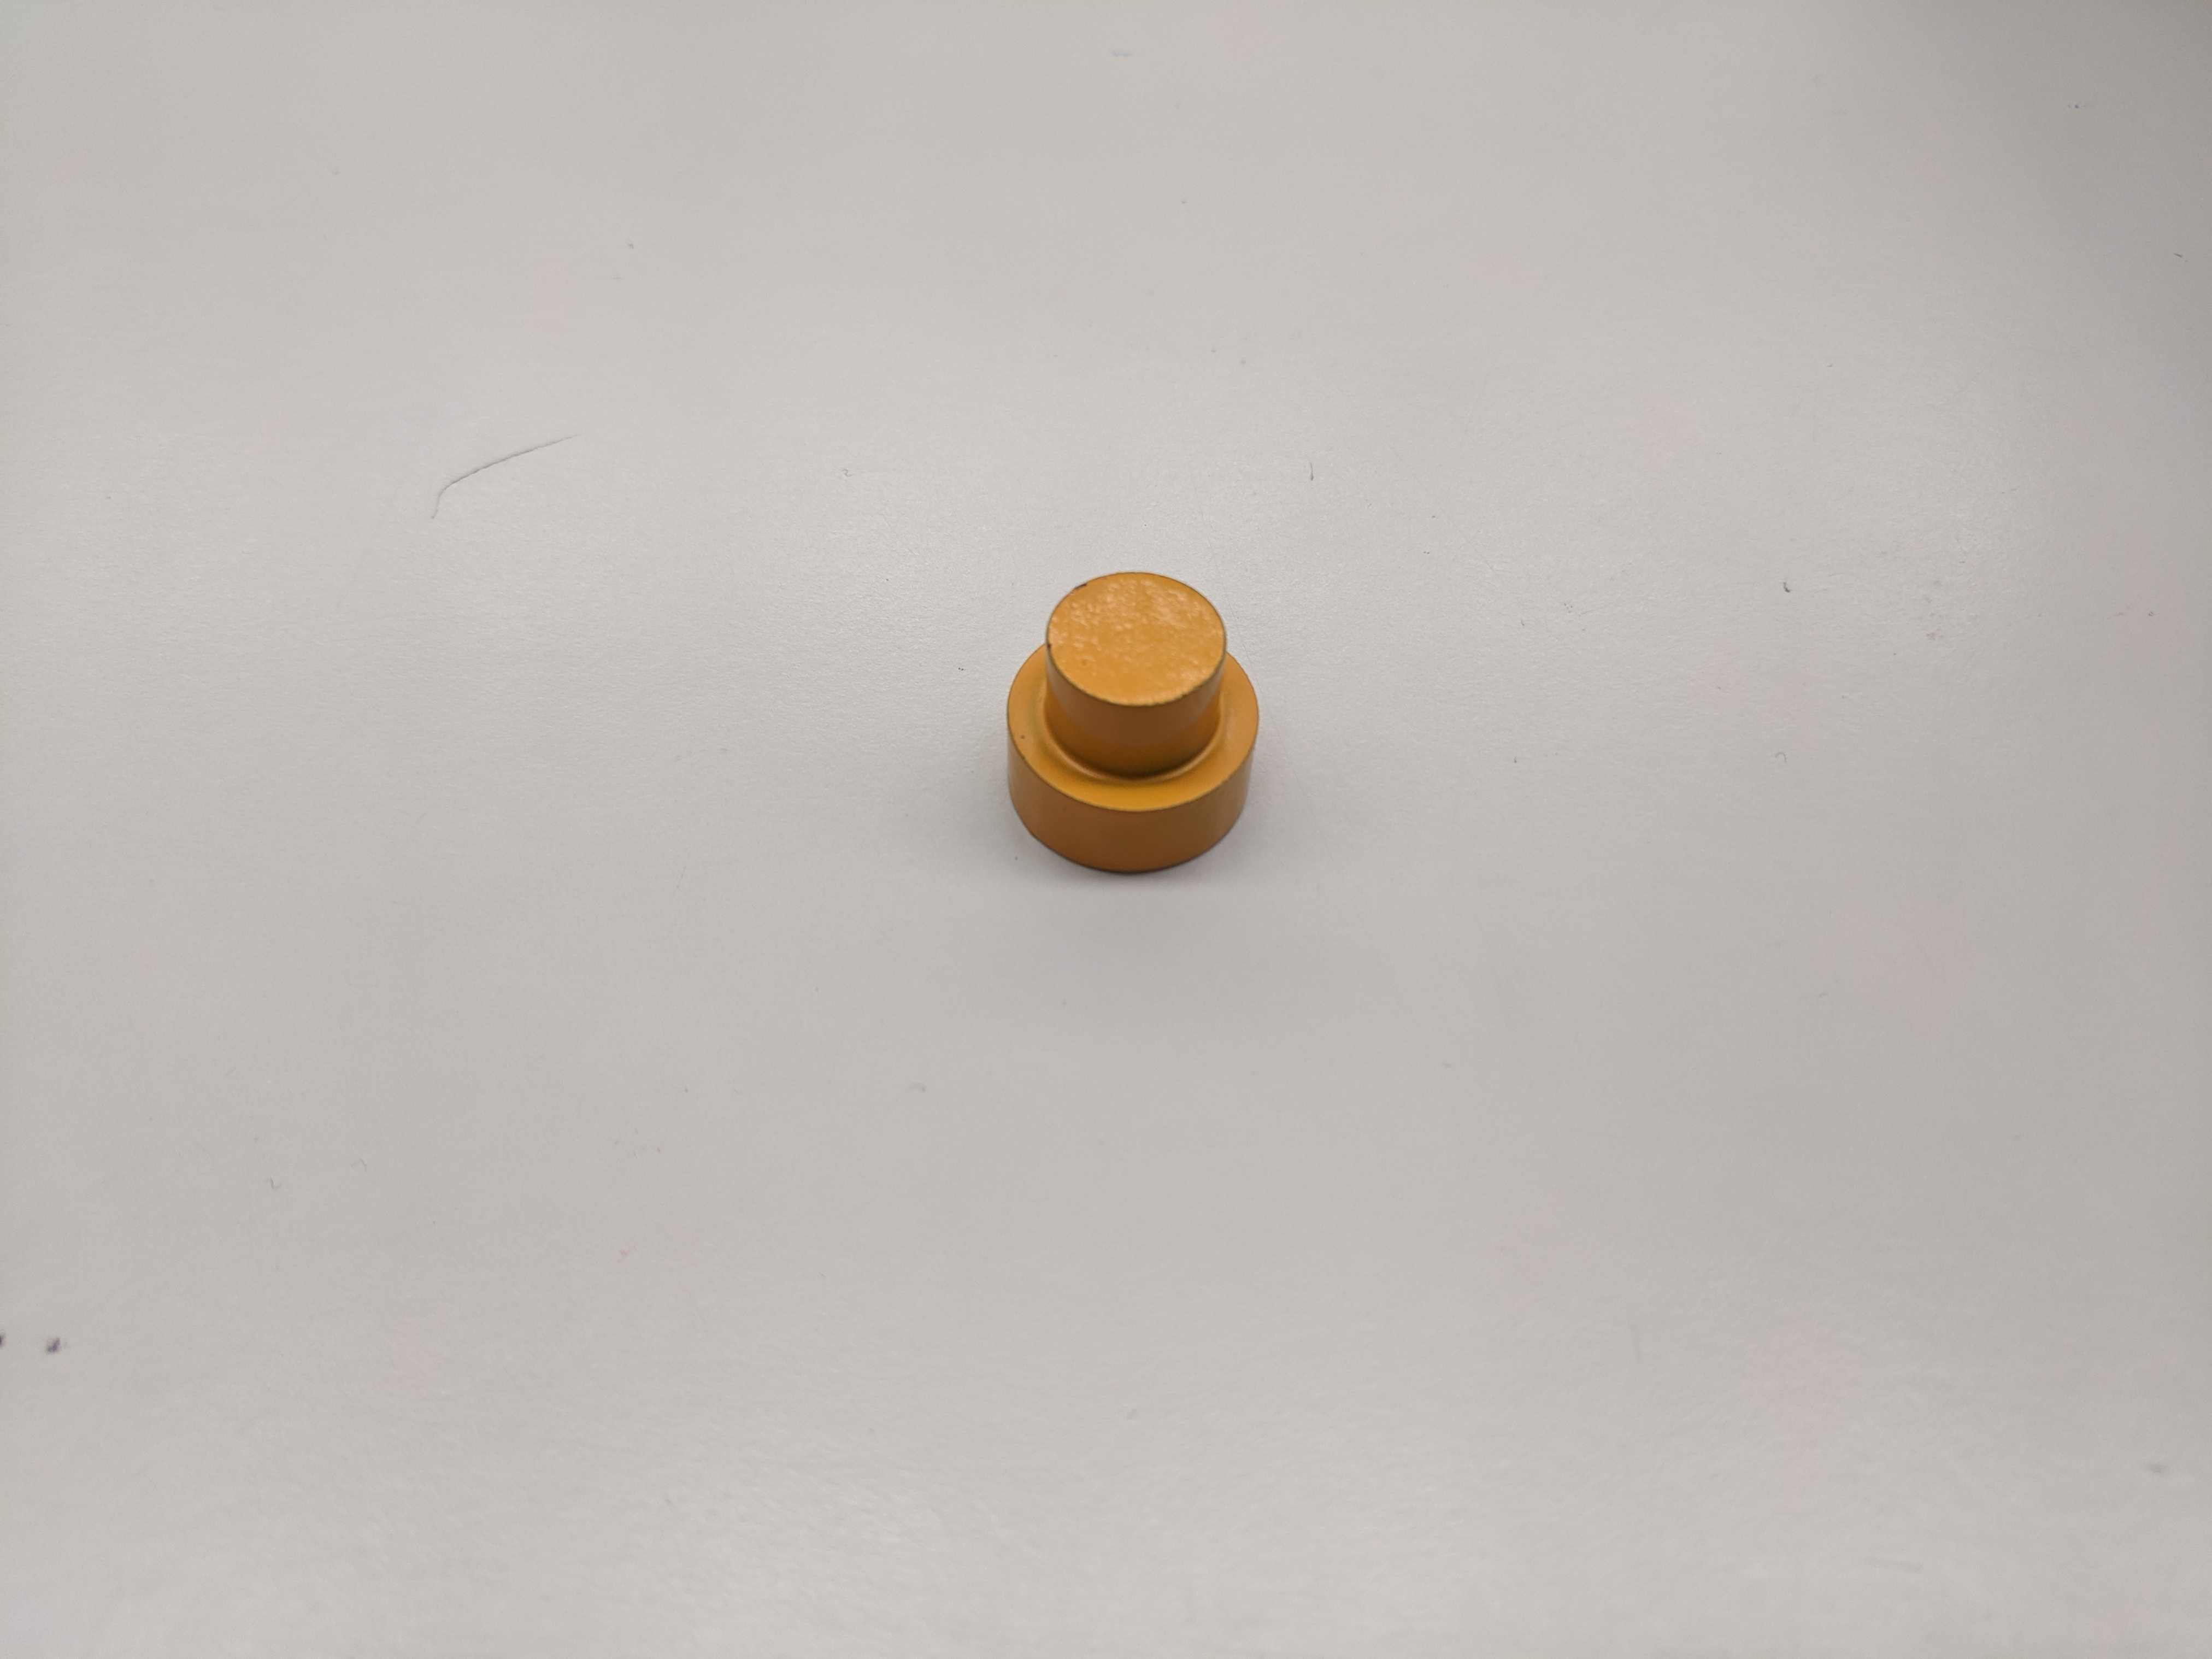
\includegraphics[scale=0.05]{scope_2}}
		\caption{The small mass that is placed in the holes cut out of the trifilar disk.}
	\end{minipage}
\end{figure}

\section{Results}
Dimensional measurements of the Trifilar were captured prior to undertaking the experiment. Measurements included disk weight $m_d$; disk radius $r_d$; filament length $L$; the radius from centre of disk to inner set of holes $d_1$ the radius from centre of disk to middle set of holes $d_2$; the radius from centre of disk to outer set of holes $d_3$; and the radius from the disk centre to the filament base $r$. These measurements are presented in Table 1 below. To better understand where the masses were mounted on the disk, the Trifilar disk geometries are shown in Figure 5.

\begin{figure}[h]
	\centering
	\begin{minipage}{0.45\textwidth}
		\centering
		\captionof{table}{Trifilar parameter measurements}
		\small
		\begin{tabular}{lrc}
			\toprule
			Description & Value & Units \\
			\midrule
			Disk Mass $(m_d)$ & 0.200 & $\si{\kilogram}$\\
			Disk Radius $(r_d)$ & 0.140 & $\si{\meter}$ \\
			Hole Radius $(r_h)$ & 0.090 & $\si{\meter}$ \\
			Filament Length $(L)$ & 0.450 & $\si{\meter}$ \\
			Distance to Inner Holes $(d_1)$ & 0.065 & $\si{\meter}$\\
			Distance to Middle Holes $(d_2)$ & 0.090 & $\si{\meter}$\\
			Distance to Outer Holes $(d_3)$ & 0.120 & $\si{\meter}$\\
			Distance to Filament $(r_F)$ & 0.049 & $\si{\meter}$ \\
			\bottomrule
		\end{tabular}
	\end{minipage}
	\hspace{1cm}
	\begin{minipage}{0.45\textwidth}
		\centering
		\captionof{table}{Dimensions of the small masses}
		\small
		\begin{tabular}{lrc}
			\toprule
			Description & Value & Units \\
			\midrule
			Object Mass $(m_{obj})$ & 0.020 & $\si{\kilogram}$ \\
			Upper Cylinder Radius $(r_u)$ & 0.009 & $\si{\meter}$ \\
			Upper Cylinder Height $(h_u)$ & 0.007 & $\si{\meter}$ \\
			Lower Cylinder Radius $(r_l)$ & 0.010 & $\si{\meter}$ \\
			Lower Cylinder Height $(h_l)$ & 0.010 & $\si{\meter}$ \\
			 & & \\
			 & & \\
			 & & \\
			\bottomrule
		\end{tabular}
	\end{minipage}
\end{figure}

\begin{figure}[h]
	\centering
	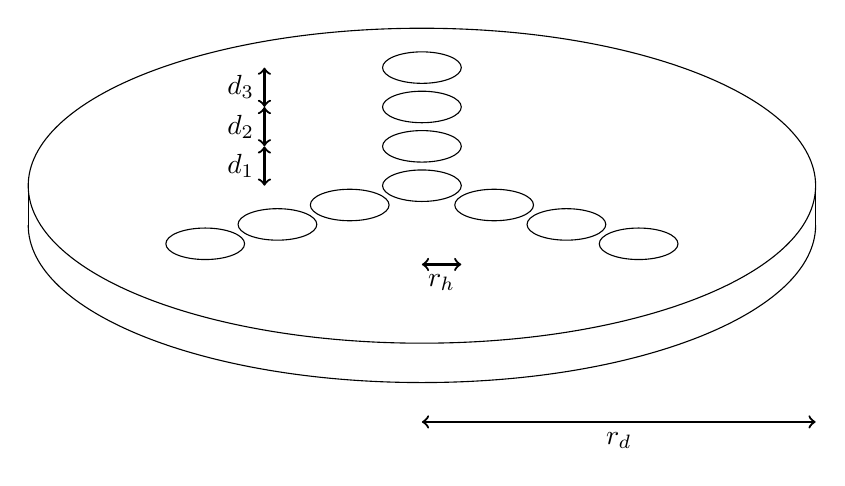
\begin{tikzpicture}
	\draw (0,0) ellipse (5 and 2);
	\draw (-5,-0.5) arc (180:360:5 and 2);
	\draw (-5,0) -- (-5,-0.5);
	\draw (5,0) -- (5,-0.5);
	
	\draw (0,0) ellipse (0.5 and 0.2);
	
	\draw (0,0.5) ellipse (0.5 and 0.2);
	\draw (0,1) ellipse (0.5 and 0.2);
	\draw (0,1.5) ellipse (0.5 and 0.2);
	
	\draw (-0.917,-0.245) ellipse (0.5 and 0.2);
	\draw (-1.835,-0.4917) ellipse (0.5 and 0.2);
	\draw (-2.752,-0.7376) ellipse (0.5 and 0.2);
	
	\draw (0.917,-0.245) ellipse (0.5 and 0.2);
	\draw (1.835,-0.4917) ellipse (0.5 and 0.2);
	\draw (2.752,-0.7376) ellipse (0.5 and 0.2);
	
	\draw[<->, thick] (0,-3) -- (5,-3) node [midway, below] {$r_d$};
	\draw[<->, thick] (0,-1) -- (0.5,-1) node [midway, below] {$r_h$};
	\draw[<->, thick] (-2,0) -- (-2,0.5) node [midway, left] {$d_1$};
	\draw[<->, thick] (-2,0.5) -- (-2,1) node [midway, left] {$d_2$};
	\draw[<->, thick] (-2,1) -- (-2,1.5) node [midway, left] {$d_3$};
	\end{tikzpicture}
	\caption{Geometries of the Trifilar disk and holes where small masses were mounted.}
\end{figure}

\vspace{0.5cm}

Measurement information was also taken about the small objects, including their mass $m_{obj}$; radius of upper cylinder $r_u$; height of the upper cylinder $h_u$; radius of the lower cylinder $r_l$; and the height of the lower cylinder $h_l$. These measurements are presented in Table 2 above. The object geometries can be seen in Figure 6.

\vspace{0.5cm}

\begin{figure}[h]
	\centering
	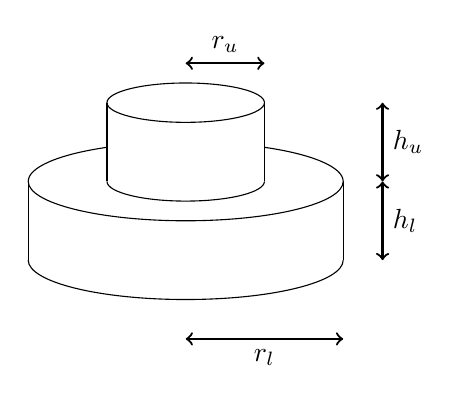
\begin{tikzpicture}
		\draw (0,0) ellipse (1 and 0.25);
		\draw (-1,-1) arc (180:360:1 and 0.25);
		\draw (-2,-1) arc (180:360:2 and 0.5);
		\draw (-2,-1) arc (180:240:2 and -0.5);
		\draw (2,-1) arc (360:300:2 and -0.5);
		\draw (-2,-2) arc (180:360:2 and 0.5);
		
		\draw (-1,0) -- (-1,-1);
		\draw (1,0) -- (1,-1);
		\draw (-2,-1) -- (-2,-2);
		\draw (2,-1) -- (2,-2);
		
		\draw [<->, thick] (0,0.5) -- (1,0.5) node [midway, above] {$r_u$};
		\draw [<->, thick] (0,-3) -- (2,-3) node [midway, below] {$r_l$};
		\draw [<->, thick] (2.5,-2) -- (2.5,-1) node [midway, right] {$h_l$};
		\draw [<->, thick] (2.5,0) -- (2.5,-1) node [midway, right] {$h_u$};
	\end{tikzpicture}
	\caption{The small objects are essentially a small cylinder stacked on top of a larger cylinder}
\end{figure}

\vspace{0.5cm}

The trifilar was rotationally perturbed and allowed to oscillate. The time taken to complete 10 oscillations was recorded. This was repeated 5 times for both the disk, and the disk with mass objects placed in the middle holes. The tabulated results can be found in Table 3. Measurement error was reduced by taking an average of results for the disk, and for the disk plus objects. Average values can be found in the final column of Table 3. 

\vspace{0.5cm}

\begin{figure}[h]
	\centering
	\captionof{table}{Five trials were undertaken to record the natural period of oscillation for 10 oscillations. This was done for both the disk, and the disk plus mass objects in the middle holes}
	\small
	\begin{tabular}{lrrrrrr}
		\toprule
		Object & $(T_{10})_1 \ [\si{\second}]$ & $(T_{10})_2 \ [\si{\second}]$ & $(T_{10})_3 \ [\si{\second}]$ & $(T_{10})_4 \ [\si{\second}]$ & $(T_{10})_5 \ [\si{\second}]$ & $(T_{10})_{avg} \ [\si{\second}]$ \\
		\midrule
		Disk & 31.91 & 31.50 & 30.97 & 30.82 & 30.78 & 31.21\\
		Disk + 3 Objects (middle) & 33.38 & 33.40 & 33.38 & 32.44 & 33.53 & 33.23 \\
		\bottomrule
	\end{tabular}
\end{figure}


\newpage

\section{Calculations}
\subsection{Moment of Inertia and Radius of Gyration for Disk}
\subsubsection{Disk experimental moment of inertia and radius of gyration}
Ten oscillations of the disk took an average time of 31.21$\si{\second}$, hence one oscillation took approximately 3.12$\si{\second}$. The natural frequency of oscillation, found using (12), is as follows:
\begin{equation}
f_n = \frac{1}{3.12} = 0.32\si{\hertz}
\end{equation}

Using equation (13) the radius of gyration was calculated as:
\begin{equation}
k_{tri} = \frac{0.049}{2 \pi \times 0.320}\sqrt{\frac{9.810}{0.450}} = 0.114\si{\meter}
\end{equation}

Using equation (14) the moment of inertia is calculated as:
\begin{equation}
(I_G)_{tri} = 2.58 \times 10^{-3} \ \si{\kilogram\meter^2}
\end{equation}

\subsubsection{Disk theoretical moment of inertia and radius of gyration}
Given that the mass of the disk is $m_d$, and letting the material area of the disk be $A$, we can specify the mass density by area for the disk material as:
\begin{equation}
	\rho_A = \frac{m_d}{A}
\end{equation}

We note that the area can be calculated by subtracting 10 small holes from the total area of the disk (refer to Figure 5 for a better understanding of disk geometry). The area $A$ can be specified as:
\begin{equation}
	A = \pi r_d^2 - 10 \pi r_h^2 = \pi (r_d^2 - 10 r_h^2)
\end{equation}

According to Meriam and Kraige \cite{Meriam:2000} the mass moment of inertia for a solid cylinder, with mass $M$ and radius $R$, about an axis running down the cylinder length through the mass centre is given by:
\begin{equation}
I = \frac{1}{2}MR^2
\end{equation}

Equation (20) can be used to determine the moment of inertia of the trifilar disk without any holes in it, around the axis through the mass centre $G$, if we assume it is a solid cylindrical object:
\begin{equation}
(I_G)_{disk} = \frac{1}{2} \rho_A (\pi r_d^2) r_d^2 = \frac{1}{2} \rho_A \pi r_d^4
\end{equation}

Similarly, we can determine the moment of inertia of a trifilar disk hole $(I_G)_{hole}$, around the axis through the mass centre $G$, if we assume it is a solid cylindrical object:
\begin{equation}
(I_G)_{hole} = \frac{1}{2} (\rho_A \pi r_h^2) r_h^2 = \frac{1}{2} \rho_A \pi r_h^4
\end{equation}

Given these assumption we calculate the moment of inertia for the trifilar disk with holes by subtracting the moments of inertia for 10 holes from (21). Note that since the holes are not all located with their axis of rotation through their mass centres, some of their moments of inertia need to be translated using the parallel axis theorm (8). Mathematically, this is expressed as: 
\begin{align}
(I_G)_{tri} = (I_G)_{disk} - (I_G)_{hole} \nonumber &- 3\big((I_G)_{hole} + \rho_A \pi r_h^2 d_1^2\big) \nonumber \\
						   &- 3\big((I_G)_{hole} + \rho_A \pi r_h^2 d_2^2\big) \nonumber \\
						   &- 3\big((I_G)_{hole} + \rho_A \pi r_h^2 d_3^2\big)
\end{align}

Substituting (21) and (22) into (23) and simplifying yields:
\begin{equation}
(I_G)_{tri} = \rho_A \pi \bigg[ \frac{1}{2} r_d^2 - 5r_h^2 - 3r_h^2 (d_1^2 + d_2^2 + d_3^3) \bigg]
\end{equation}

Hence, substituting the values from Tables 1 and 2 into (24) yields:
\begin{equation}
	(I_G)_{tri} = 2.56 \times 10^{-3} \ \si{\kilogram\meter^2}
\end{equation}

Finally, we can simply employ (9) to find the theoretical radius of gyration:
\begin{equation}
	k_{tri} = \sqrt{\frac{2.56 \times 10^{-3}}{0.2}} = 0.113 \si{\meter}
\end{equation}

\subsection{Moment of Inertia and Radius of Gyration for Disk and Objects}
\subsubsection{Disk and objects experimental moment of inertia and radius of gyration}
Ten oscillations of the disk plus the three objects located in the middle holes took an average time of 33.23$\si{\second}$, hence one oscillation took approximately 3.32$\si{\second}$. Similarly to Section 3.1.1, the natural frequency of oscillation is found using (12) and is:
\begin{equation}
f_n = \frac{1}{3.32} = 0.30\si{\hertz}
\end{equation}

Using equation (13) the radius of gyration was calculated as:
\begin{equation}
k_{tri\_and\_3\_obj} = \frac{0.049}{2 \pi \times 0.30}\sqrt{\frac{9.810}{0.450}} = 0.121\si{\meter}
\end{equation}

Using equation (14) the moment of inertia is calculated as:
\begin{equation}
(I_G)_{tri} + 3(I_O)_{obj} = 0.121^2 (0.2 + 3 \times 0.02) = 3.83 \times 10^{-3} \ \si{\kilogram\meter^2}
\end{equation}

\subsubsection{Disk and objects theoretical moment of inertia and radius of gyration}
Given that the mass of one of the objects is $m_{obj}$, and letting the volume of the object be $V$, we can specify the mass density by volume for the objects as:
\begin{equation}
	\rho_V = \frac{m_{obj}}{V}
\end{equation}

We note that the volume can be calculated by considering the object as two small cylinders, which yields:
\begin{equation}
	V = \pi (r_u^2 h_u + r_l^2 h_l)
\end{equation}

Additionally, considering the mass as two solid cylinders allows us to employ equation (20) to determine the moment of inertia about the axis through the mass centre for a single object:
\begin{equation}
	(I_G)_{obj} = \frac{1}{2} (\rho_V \pi r_u^2 h_u) r_u^2 + \frac{1}{2} (\rho_V \pi r_l^2 h_l) r_l^2 
\end{equation}

Simplifying equation (32) yields:
\begin{equation}
	(I_G)_{obj} = \frac{1}{2} \rho_V \pi (r_u^4 h_u + r_l^4 h_l)
\end{equation}

Now, we want to determine the moment of inertia for the trifilar disk and the three mass objects. First we need to translate the result in (33) to a parallel axis. Using (8) we get:
\begin{equation}
	(I_O)_{obj} = (I_G)_{obj} + m_{obj} \times d_2^2
\end{equation}

Finally, using our theoretical result for the moment of inertia of the trifilar disk from Section 3.1.2, we can evaluate the moment of inertia for the disk plus three objects in the middle holes using the expression in (34). This yields:
\begin{equation}
	(I_G)_{tri} + 3(I_O)_{obj} = (I_G)_{tri} + 3 \big( (I_G)_{obj} + m_{obj} \times d_2^2 \big) = 3.06 \times 10^{-3} \ \si{\kilogram\meter^2}
\end{equation}

Finally, we can again employ (9) to determine the radius of gyration:
\begin{equation}
	k_{tri\_and\_3\_obj} = \sqrt{\frac{3.06 \times 10^{-3}}{0.2 + 3 \times 0.02}} = 0.108 \si{\meter}
\end{equation}

\section{Discussion}
The experimental and theoretical results for the moments of inertia and radius of gyration calculated in Sections 3.1.1, 3.1.2, 3.2.1, and 3.2.2 are summarised in Table 4. Calculated results from experimental data are greater than theoretical values for the disk, but only marginally. Experimental moment of inertia for the disk is 0.78\% greater than the theoretical value. Similarly, the experimentally determined radius of gyration is 0.88\% greater than the theoretical result. The tiny differences in magnitude suggest that experimentally determining the moment of inertia and radius of gyration for the unloaded trifilar disk is reasonably accurate. Further, these differences are most likely explained by stochastic measurement error when timing the disk oscillations, or something similar.  
\begin{table}[h]
	\centering
	\caption{Summary of the key results from Sections 3.1.1, 3.1.2, 3.2.1, and 3.2.2}
	\begin{tabular}{lrrrrrr}
		\toprule
		& \multicolumn{3}{c}{Moment of Inertia} & \multicolumn{3}{c}{Radius of Gyration} \\
		\cmidrule(l{3pt}r{3pt}){2-4} \cmidrule(l{3pt}r{3pt}){5-7}
		Description & Experimental & Theoretical & Error & Experimental & Theoretical & Error\\
		 & \multicolumn{1}{c}{$[\si{\kilogram\meter^2}]$} & \multicolumn{1}{c}{$[\si{\kilogram\meter^2}]$} & \multicolumn{1}{c}{$[\%]$} & \multicolumn{1}{c}{$[\si{\meter}]$} & \multicolumn{1}{c}{$[\si{\meter}]$} & \multicolumn{1}{c}{$[\%]$} \\ 
		\midrule
		Disk & $2.58 \times 10^{-3}$ & $2.56 \times 10^{-3}$ & 0.78 & 0.114 & 0.113 & 0.88 \\
		Disk + 3 objects & $3.83 \times 10^{-3}$ & $3.06 \times 10^{-3}$ & 25.16 & 0.121 & 0.108 & 12.04\\
		\bottomrule
	\end{tabular}
\end{table}

Loading the disk's middle holes with three masses inflated the difference between experimental and theoretical values for the moment of inertia and radius of gyration. Indeed, the experimental moment of inertial was 25.16\% bigger than the theoretical value. Similarly, the experimental radius of gyration was 12.04\% bigger than the theoretical value. The increase in difference is most likely due to model error brought about as the system mass increases. Formulas used for the experimental calculations were derived by considering system forces which produced a second order, ordinary differential equation. The solution of this ode resulted in an undamped oscillatory response. Of course in reality the rig violates this assumption since frictions on trifilar filaments would act as system dampners. It may be the case that an increase of mass also increases the friction on filaments. 

\section{Conclusion}
The trifialr rig would work well for calculating moments of inertia and the radius of gyration for objects which do not changes the mass of the system very much, however, the rig only works semi-reliably for objects of 60$\si{g}$ of more. Experimentally calculated moments of inertia were 25\% greater than the theoretical values for a 60$\si{g}$ mass symmetrically distributed over the trifilar plate. Similarly, the experimentally calculated radius of gyration was 12\% greater than the theoretical value. The divergent results are most likely due to model error since there is an undamped oscillation assumption used in experimental calculations. Collection of more experimental values for different masses may help to identify a trend in the error. This future work may allow for the development of systematic correction factors which could be applied to get accurate moments of inertia and radius of gyration.     

\bibliography{my_bib}
\bibliographystyle{ieeetr}

\end{document}